\section{VIEWR}
\label{sVIEWR}

\hypertarget{sVIEWRhy}{The}
VIEWR module provides a general-purpose plotting capability for
NJOY.  It reads in user commands that define a variety of 2-D and
3-D graphs, and then it writes a Postscript file to display the
graphs with high quality.  Some of the capabilities of VIEWR include
\index{plotting}
\index{VIEWR|textbf}

\begin{itemize}
\begin{singlespace}
\item conventional 2-D plots (for example, cross section {\it vs} energy)
      with the normal combinations of linear and log scales, automatic
      or user-specified ranges and labels, an optional alternate
      right-hand axis, and with one or two title lines;

\item curves of various line patterns, labeled with tags and arrows
      or described in a legend block;

\item data points given with a variety of symbols with error bars (they
      can be identified in a legend block);

\item the superposition of several plots on a given set of axes;

\item detailed 3-D perspective plots for data such as angular
      distributions or energy distributions, with a choice of linear
      or log axes, with a choice of working area and viewpoint, and
      with one or two title lines;

\item color can be used to distinguish between different curves, and
      the graphics window area and page background can also have
      selected colors;

\item closed regions can be displayed with various kinds of cross
      hatching for filled with selected colors; and

\item multiple plots can be put on each page.
\end{singlespace}
\end{itemize}

\noindent
Many examples of graphs generated by VIEWR can be found elsewhere in
this report.

This chapter describes the VIEWR module in NJOY2016.0.

\subsection{Modular Structure}
\label{ssVIEWR_mod}

The \cword{viewr}\index{viewr@{\ty viewr}}
subroutine is encapsulated into a Fortran-90 module
that only makes public that one subroutine call.  This module is
supported by module \cword{graph}\index{modules!graph@{\ty graph}},
which makes a number of calls and data structures public.  The
features in \cword{graph} provide the low-level capabilities for
generating Postscript graphics that are used by the routines
in VIEWR.  We will first describe VIEWR by giving the user-input
specifications and describing the details of the VIEWR coding.
 Finally, we will describe the details of the graphics
calls as implemented in the separate \cword{graph} module.

\subsection{Using VIEWR}
\label{ssVIEWR_using}

The VIEWR module can be used as a general-purpose plotting engine by
constructing input for it by hand.  However, it is more commonly used
to display data assembled by other NJOY modules.  For example,
\hyperlink{sPLOTRhy}{PLOTR}\index{PLOTR} reads data
in ENDF, PENDF\index{PENDF}, or
GENDF\index{GENDF} formats and constructs an output file in VIEWR
format.  \hyperlink{sCOVRhy}{COVR}\index{COVR} constructs
an elaborate set of plots of
cross-section covariance data using color contour maps and rotated
subplots.  \hyperlink{sHEATRhy}{HEATR}\index{HEATR} can
produce graphs showing the heating
value, the photon energy production, and their associated kinematic
limits.   \hyperlink{sDTFRhy}{DTFR}\index{DTFR} and
\hyperlink{sACERhy}{ACER}\index{ACER} both are capable of
generating VIEWR files that show the cross sections and distributions
contained in the libraries that they produce.  See the writeups for
these various modules for examples of these kinds of plots.


\subsection{Input Instructions}
\label{ssVIEWR_inp}
\index{VIEWR!VIEWR input}
\index{input!VIEWR}

There is actually only one line of input for the VIEWR module itself:

\small
\begin{ccode}

   !---input--------------------------------------------------------
   !
   !  card 1
   !     infile        input file
   !     nps           postscript output file
   !

\end{ccode}
\normalsize

\noindent
The plotting commands and data are provided on an input file to VIEWR
that use the following format:

\small
\begin{ccode}

   !---data file format---------------------------------------------
   !
   !  card 1
   !     lori          page orientation (def=1)
   !                    0  portrait (7.5x10in)
   !                    1  landscape (10x7.5in)
   !     istyle        character style (def=2)
   !                     1  roman
   !                     2  swiss
   !     size          character size option
   !                     pos = height in page units
   !                     neg = height as fraction of subplot size
   !                       (default=.30)
   !     ipcol         page color (def=white)
   !                    0=white
   !                    1=navajo white
   !                    2=blanched almond
   !                    3=antique white
   !                    4=very pale yellow
   !                    5=very pale rose
   !                    6=very pale green
   !                    7=very pale blue
   !
   ! -----repeat cards 2 through 13 for each curve-----
   !
   !  card 2
   !     iplot         plot index
   !                     99 = terminate plotting job
   !                      1 = new axes, new page
   !                     -1 = new axes, existing page
   !                      n = nth additional plot on existing axes
   !                     -n = start a new set of curves using
   !                          the alternate y axis
   !                     default = 1
   !     iwcol         window color (def=white)
   !                    color list same as for ipcol above
   !     factx         factor for energies (default=1.)
   !     facty         factor for cross-sections (default=1.)
   !     xll,yll       lower-left corner of plot area
   !     ww,wh,wr      window width, height, and rotation angle
   !                   (plot area defaults to one plot per page)
   !
   ! -----cards 3 thru 7 for iplot = 1 or -1 only-----
   !
   !  card 3
   !     t1            first line of title
   !                   60 characters allowed.
   !                   default=none
   !
   !  card 3a
   !     t2            second line of title
   !                   60 characters allowed.
   !                   default=none
   !
   !  card 4
   !     itype         type for primary axes
   !                     1 = linear x - linear y
   !                     2 = linear x - log y
   !                     3 = log x - linear y
   !                     4 = log x - log y
   !                     set negative for 3d axes
   !                     0 = no plot, titles only
   !                     default=4
   !     jtype         type for alternate y axis or z axis
   !                     0 = none
   !                     1 = linear
   !                     2 = log
   !                     default=0
   !     igrid         grid and tic mark control
   !                     0 = no grid lines or tic marks
   !                     1 = grid lines
   !                     2 = tic marks on outside
   !                     3 = tic marks on inside
   !                     default=2
   !     ileg          option to write a legend.
   !                     0 = none
   !                     1 = write a legend block with upper left
   !                         corner at xtag,ytag (see below)
   !                     2 = use tag labels on each curve with
   !                         a vector from the tag to the curve
   !                     default=0
   !     xtag          x coordinate of upper left corner
   !                   of legend block
   !     ytag          y coord of upper left corner
   !                   default=upper left corner of plot
   !
   !  card 5
   !     xmin          lowest energy to be plotted
   !     xmax          highest energy to be plotted
   !     xstep         x axis step
   !                   default = automatic scales
   !                   (for linear, give all 3, or none)
   !                   (for log, give first 2, or none)
   !
   !  card 5a
   !     xlabl         label for x axis
   !                   60 characters allowed.
   !                   (default = no label, no numbering)
   !
   !  card 6
   !     ymin          lowest value of y axis.
   !     ymax          highest value of y axis.
   !     ystep         step for y ayis (linear scales only)
   !                   default = automatic scales
   !                   (for linear, give all 3, or none)
   !                   (for log, give first 2, or none)
   !
   !  card 6a
   !     ylabl         label for y axis
   !                   60 characters allowed.
   !                   (default = no label, no numbering)
   !
   !  card 7   (jtype.gt.0 only)
   !     rmin          lowest value of secondary y axis or z axis
   !     rmax          highest value of secondary y axis or z axis
   !     rstep         step for secondary y axis or z axis
   !                   (default = automatic scale)
   !                   (for linear, give all 3, or none)
   !                   (for log, give first 2, or none)
   !
   !  card 7a  (jtype.gt.0 only)
   !     rl            label for alternate y axis or z axis
   !                   60 characters allowed.
   !                   (default = no label, no numbering)
   !
   !   card 8  -- dummy input card for consistency with plotr
   !               it always should be 0/
   !
   ! -----cards 9 and 10 for 2d plots only-----
   !
   !   card 9
   !     icon          symbol and connection option
   !                     0 = points connected, no symbols
   !                    -i = points not connected, symbol at every
   !                         ith point
   !                     i = points connected, symbol at every ith
   !                         points
   !                     default=0
   !     isym          no. of symbol to be used
   !                     0 = square
   !                     1 = octagon
   !                     2 = triangle
   !                     3 = cross
   !                     4 = ex
   !                     5 = diamond
   !                     6 = inverted triangle
   !                     7 = exed square
   !                     8 = crossed ex
   !                     9 = crossed diamond
   !                     10 = crossed octagon
   !                     11 = double triangle
   !                     12 = crossed square
   !                     13 = exed octagon
   !                     14 = triangle and square
   !                     15 = filled circle
   !                     16 = open circle
   !                     17 = open square
   !                     18 = filled square
   !                     19 = filled diamond
   !                     20 = filled triangle
   !                     21 = filled inverted triangle
   !                     22 = crossed circle
   !                     23 = exed circle
   !                     24 = exed diamond
   !                     default=0
   !     idash         type of line to plot
   !                     0 = solid
   !                     1 = dashed
   !                     2 = chain dash
   !                     3 = chain dot
   !                     4 = dot
   !                     5 = invisible
   !                     default=0
   !     iccol         curve color (def=black)
   !                     0=black
   !                     1=red
   !                     2=green
   !                     3=blue
   !                     4=magenta
   !                     5=cyan
   !                     6=brown
   !                     7=purple
   !                     8=orange
   !     ithick        controls thickness of curve
   !                     0 = invisible (for shaded areas)
   !                     (default=1)
   !     ishade        shade pattern
   !                     0 = none
   !                     1 to 10 = 10\% to 100\% gray
   !                     11 to 20 = 45 deg right hatching
   !                     21 to 30 = 45 deg left hatching
   !                     31 to 40 = 45 deg cross hatching
   !                     41 to 50 = shades of green
   !                     51 to 60 = shades of red
   !                     61 to 70 = shades of brown
   !                     71 to 80 = shades of blue
   !                     default=0
   !
   !   card 10   ---ileg.ne.0 only---
   !     aleg          title for curve tag or legend block
   !                   60 characters allowed.
   !                   default=blank
   !
   !   card 10a  ---ileg.eq.2 only---
   !     xtag          x position of tag title
   !     ytag          y position of tag title
   !     xpoint        x coordinate of vector point
   !                    (.le.0 to omit vector)
   !
   ! -----card 11 for 3d plots only-----
   !
   !   card 11
   !     xv,yv,zv      abs. coords of view point
   !                   defaults= 15.,-15.,15.
   !     x3,y3,z3      abs. sides of work box volume
   !                   defaults=2.5,6.5,2.5
   !
   !          set x3 negative to flip the order of the axis on
   !          that side of the box (secondary energy, cosine).
   !
   !   card 12
   !     nform          format code for input data
   !                    0 = free format input with
   !                        optional x and y error bars
   !                    1 = free format input for a
   !                        3d family of curves z(x) vs y
   !
   !   card 13   ---nform = 0 only---   2-d data
   !     xdata          independent value
   !                    terminate with empty card (/)
   !     ydata          dependent value
   !     yerr1          lower y error limit
   !                    no y error bar if zero
   !     yerr2          upper y error limit
   !                    if zero, equals yerr1
   !     xerr1          x left error limit
   !                    no x error bar if zero
   !     xerr2          x right error limit
   !                    if zero, equals xerr1
   !
   !   card 14   ---nform = 1 only---   3-d data
   !     y              y value for curve
   !                    repeat cards 13 and 13a for each curve
   !                    terminate with empty card (/)
   !
   !   card14a   ---nform = 1 only---
   !     x              x value
   !     z              z value
   !                    repeat card 13a for each point in curve
   !                    terminate with empty card (/)
   !                    disspla version requires same x grid
   !                    for each value of y.
   !
   !--------------------------------------------------------------------

\end{ccode}
\normalsize

Card 1 in the data file format sets up the specifications for the
graphics page.  The orientation can be either portrait or landscape.
Characters can use a serif style ``roman,'' implemented by the
Postscript Times-Roman font, or sans-serif ``swiss,'' implemented
by the Postscript Helvetica font.  The character size can be specified
in inches or as a fraction of the subplot size.  The latter is handy
when subplots are shrunk down to just a fraction of the page.  The
default character size is 0.30 inches.  The page color set here is the
color of the overall page.  See below for the color inside the frame
of a subplot.  We have provided a set of pale colors here for these
backgrounds.

Card 2 starts a new plot, subplot, or curve on an existing plot.  It
also provides the flag indicating the the plotting job is finished;
namely, \cword{iplot}=99/.  The value for \cword{n} when its magnitude
is greater than one is arbitrary, but we often use 2, 3, {\it etc.},
to indicate the second, third, {\it etc.}, curves on a set of axes.
You could just use the value \cword{n}=2 for every additional curve,
and it would still work.  The window color \cword{ipcol} refers to
the color inside the axes frame for 2-D plots and to the color used
for the various slices of the function for 3-D plots.  The same set
of light colors described for the page background is used here, and
the pages look good if different colors are selected for the page
color and the window color.  The parameters \cword{factx} and
\cword{facty} are handy for changing the x or y units for a plot
or for scaling curves on a multi-curve graph to be closer to
each other.  The last few parameters on this card are only needed
when several small subplots are put onto one page.  They define the
position, size, and rotation of the subplot.  The covariance plots
from \hyperlink{sCOVRhy}{COVR} make use of this feature.

The next few lines of input are only given for new plots or subplots.
There can be zero, one, or two lines of titles provided above the
graph.  The size of the plot readjusts to use the space not used by
titles.  The titles (and all the other labels in VIEWR) can use some
special characters to trigger effects like subscript, superscript,
symbol characters, size changes, or font changes.  The rules for
this are defined in the source listing as follows:

\small
\begin{ccode}

   !
   ! Character specifications are similar to DISSPLA, except that
   ! the default case is lower instead of upper.  This allows
   ! mixed-case strings to be used in Postscript mode.  The
   ! following shift characters are used:
   !     < = upper-case standard
   !     > = lower-case or mixed-case standard
   !     [ = upper-case greek
   !     ] = lower-case or mixed-case greek
   !     # = instructions
   ! Give one of the shift characters twice to get it instead of
   ! its action.  The following instructions are supported:
   !     Ev = elevate by v as a fraction of the height
   !           if v is missing or D is given, use .5
   !     Lv = lower by v as a fraction of the height
   !           if v is missing or D is given, use .5
   !     Hv = change height by v as a fraction of the height
   !           if v is missing or D is given, use .5
   !     Fi = change to font number i
   !     Mi = change mode number, where mode 0 is the lower 128
   !           postscript characters and mode 1 is the upper 128
   !     X  = reset E, L, or H.  Font and Mode must be
   !           reset explicitly.
   !     c is a real number, i is an integer.
   !

\end{ccode}
\normalsize

\noindent
Normal characters are just entered using mixed upper and lower case
as desired.  If desired, upper case can be forced using the trigger
character.  For example,

\small
\begin{ccode}

   <p>u-239 from <endf/b-vi>

\end{ccode}
\normalsize

\noindent
will have the indicated characters displayed in upper case.  Similarly,
Greek letters can be entered using mixed upper and lower case, or they
can be given in all lower case and then forced to upper case with the
trigger character:

\small
\begin{ccode}

   Display ]a> and ]b>, then ]G> and ]D>
   Display ]a< and ]b>, then [g> and [d>

\end{ccode}
\normalsize

\noindent
Subscripts and superscripts use the ``instruction'' trigger character.
For example,

\small
\begin{ccode}

   ENDF/B-VI #EH<3#HXEX<h>e

\end{ccode}
\normalsize

\noindent
displays the isotope name for $^3$He correctly with a subscript one-half
the size of the main characters.  Subscripts lowered by one-quarter of
the character size and with height equal to three-quarters of the
character size could be obtained using

\small
\begin{ccode}

  X#L.25H.75<min#HXLX<

\end{ccode}
\normalsize

\noindent
For the mapping of the symbols and the other special characters available
by shifting to the upper 128 characters in each font, check the Postscript
Red Book\cite{redbook}.

Returning to the input data, Card 4 sets up the axes for the plot
using \cword{itype} and \cword{jtype}.  Several choices are allowed
for adding grid lines to the axes.  There are two ways available
to label the curves in multi-curve graphs, namely, legend blocks, and
curve tags.  The default location for the legend block is the upper
left corner of the graph area, but it can be positioned wherever
desired using \cword{xtag} and \cword{ytag}.  These values use
coordinate units.  The legend block contains a line for each curve
giving the plotting symbol, curve style or color, and an identifying
string entered below (see \cword{aleg}).  Curve tags are defined
below.

Cards 5, 5a, 6, 6a, 7, and 7a define the axis limits, step sizes, and
labels.  The limits and step sizes are defined automatically based
on the data, but they can also be defined manually to better control
the display.  This is often necessary for multi-curve plots, because
the axes are chosen based on the extent of the first curve, which may
not be suitable for all the curves in the graph.  The graph scales
are sometimes scaled with a power of ten, and these powers are
always chosen to be divisible by three.  Thus, you might have a
scale labeled barns with a factor of $10^{-3}$ indicated; the numbers
on the scale would then by milli-barns.  Note that when no label is
given, the numbering for the axis is also omitted.

Card 8 is a dummy card that is only used to make the VIEWR input
more compatible with the \hyperlink{sPLOTRhy}{PLOTR}
input.  As indicated, it should always contain \cword{0/}.

Cards 9, 10, and 10a are used for curves on 2-D plots.  You an use
the \cword{icon} connection parameter to choose simple curves, sets of
symbols, or symbols connected by curves.  A variety of symbols and curve
types are provided, and curves can be rendered in color if desired.  The
colors provided are all darker than the light backgrounds provided.  We
do not allow for the light curves on dark backgrounds that some people
like.  Another way to distinguish between different curves is with the
weight of the curve (see \cword{ithick}).  If the curve being plotted is
closed, it can be filled with hatching patterns, shades of gray, or
colors (shades of green, red, brown, or blue).  The shades of gray could
be used to show a variance band around a curve.  The colors are used
for the contour plots of covariances produced by
\hyperlink{sCOVRhy}{COVR}, and many other
uses are possible.  See Fig.~\ref{fills} for examples of fills.

\begin{figure}[t]\centering
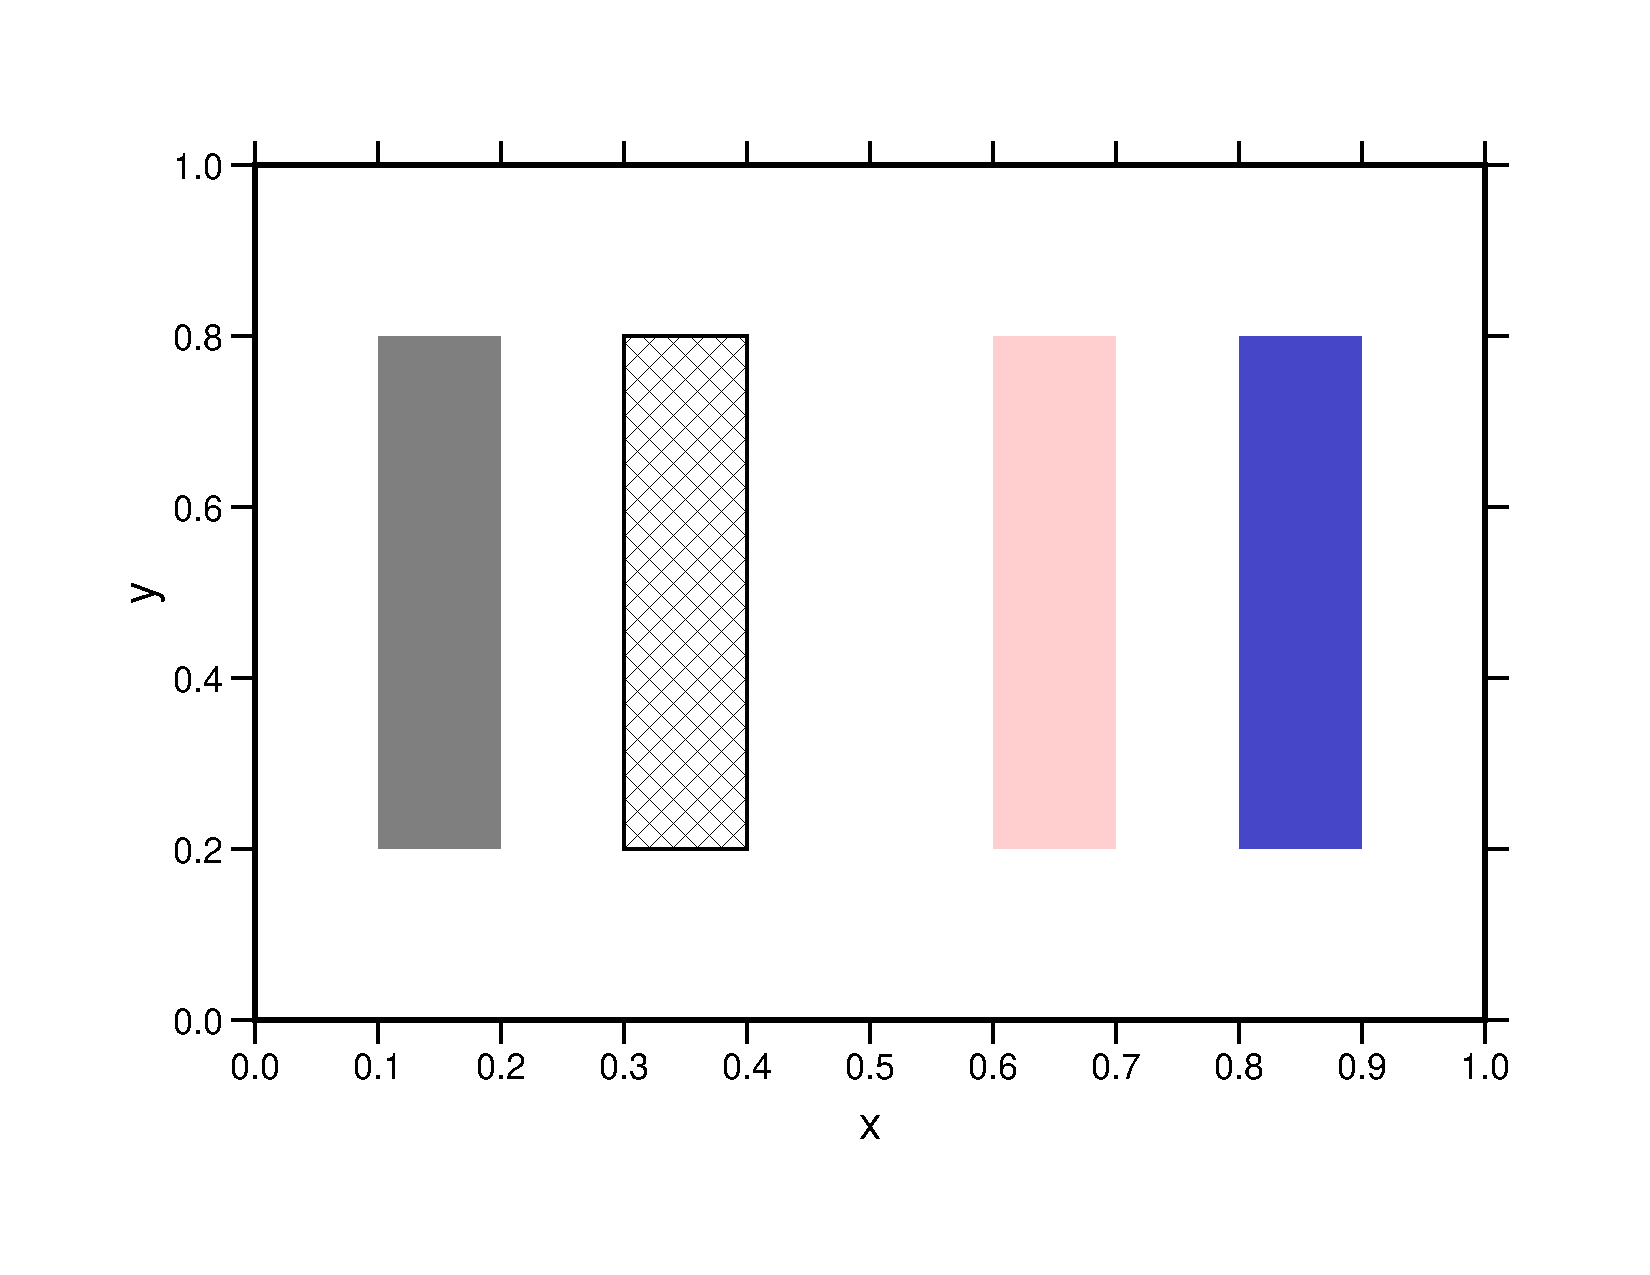
\includegraphics[keepaspectratio, height=3.5in, angle=0]{figs/fillsack}
\caption[Sample region fill options in VIEWR]{Examples of regions filled
 with gray, cross hatching and outlined, pink, and dark blue.}
\label{fills}
\end{figure}

Card 10 gives \cword{aleg}, the identifying string
for the curve that is used if legend blocks or curve tags were requested.
The location for the curve tag and the point where the arrow point touches
the curve are defined on Card 10a.  The arrow from the tag to the curve
can be omitted, if desired.

Card 11 is only given for 3-D plots.  It defines the imaginary work
box that contains the perspective view of the 3-D function, and it
defines the view point outside of the box where your eye goes.  The
perspective distortion will be greater for close viewpoints and less
for distant ones.  The 3-D coding is not very sophisticated, and it
is best to keep the view point in the octant defined by the defaults
x,y,z=(15,-15,15).  That is, you are looking in along the x and z
axes and the y axis is running away from you.  You have the option
of flipping the sense of the x axis, which is along the front of
the work box as seen from the view point.  This makes it possible
to see features on either side of the slices of the function that
are given for different discrete values of y.  Fig.~\ref{axes} may
help to clarify the coordinate system used.

\begin{figure}[thb]\centering
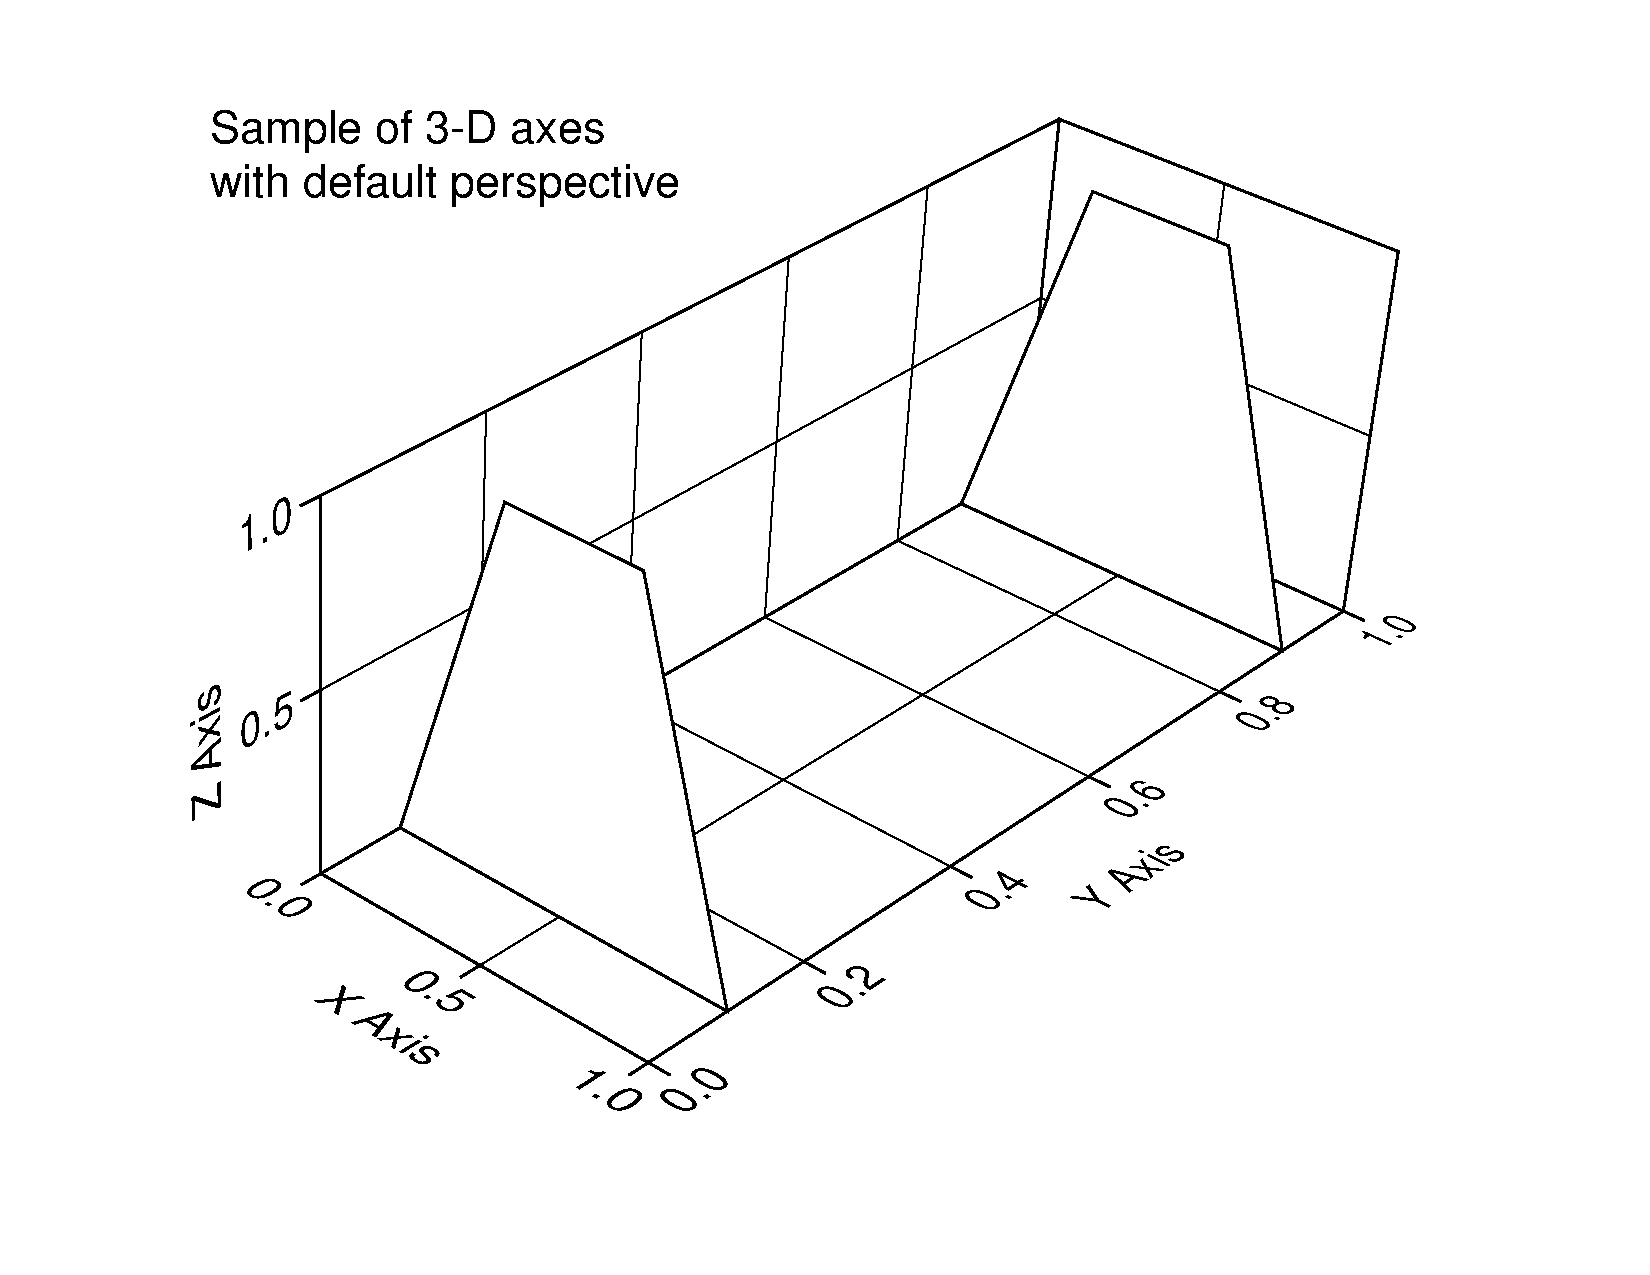
\includegraphics[keepaspectratio, height=3.5in, angle=0]{figs/viewr1ack}
\caption[Sample 3-D plot with default axis and perspective]{The 3-D
 coordinate system using the default work box and view point.}
\label{axes}
\end{figure}

At this point, all the specifications for the 2-D or 3-D graph have
been entered, and it is only necessary to enter the actual values to
be plotted.  The format to be used is controlled by \cword{nform},
which currently has only two options.  Option \cword{nform}=0 is
used for 2-D curves with optional error bars.  In order to make
the input simple for simple cases, the sequence of the possible
x and y values is arranged to be defaulted at various points.  For
a simple curve, you can just give x and y, and then terminate the
line with /.  For the most common case of error bars (symmetric y
errors), just give x, y, delta-y, and the terminating slash.  The next
step allows for asymmetric y error bars, then symmetric x error bars,
and finally asymmetric x error bars.  Terminate the list with an empty
line (only /).

For 3-D views, the function is represented by giving a set of curves
$z(x)$ for given values of $y$.  The $y$ values are given in
increasing order, and each $y$ value is followed by lines of
$x$ and $z$ values terminated by /.  The set of lines for each $y$ is
terminated by an empty card (only /).  The $y$ list is also terminated
by an empty line, so there are two lines with only / given at the end
of the \cword{nform}=1 structure.

After the input data are given, the code loops back to search for
another \cword{iplot} value.  If \cword{iplot}=99, the job is finished.


\subsection{Coding Details}
\label{ssVIEWR_details}

The main entry for VIEWR is subroutine
\cword{viewr}\index{viewr@{\ty viewr}}, which is
exported by module \cword{viewm}.\index{modules!viewm@{\ty viewm}}
It starts up by setting the default values for paper size, margins,
font size, line width, work box, and viewpoint.  Sizes are currently
given in inches (with apologies to the rest of the world).  The first
part of the input is read in to determine the page parameters, and then
subroutine \cword{gplot}\index{gplot@{\ty gplot}} from the \cword{graph}
module\index{modules!graph@{\ty graph}}
is called to initialize the plotting system.

The next step is to start the main loop over various plots, subplots,
and curves in plots.  The key to this is \cword{iplot}, and this
loop continues until \cword{iplot}=99.  For other values of
\cword{iplot}, the code reads in the user's input and stores the
values in global variables for the \cword{viewm} module.  When all
of the input values have been read for this particular plot, subplot,
or curve, subroutine \cword{viewr} call either
\cword{set2d}\index{set2d@{\ty set2d}} or
\cword{set3d}\index{set3d@{\ty set3d}}
to do the work, and then loops back for the next case.
When it sees \cword{iplot}=99, it closes the current window
(\cword{endw}\index{endw@{\ty endw}}), closes the current page
(\cword{endp}\index{endp@{\ty endp}}), shuts down the
plotting system (\cword{gdone}\index{gdone@{\ty gdone}}),
and exits from the VIEWR module.

Subroutine \cword{set2d} is used to prepare a 2-D plot or subplot,
\index{set2d@{\ty set2d}}
or to add another curve to an existing set of 2-D axes.  The information
on the particular curve being plotted is passed in as parameters to the
subroutine, and the other parameters that describe the plot or curve
are available in the global variables (see the beginning of module
\cword{viewm}).  For new plots, the code calls
\cword{initp}\index{initp@{\ty initp}} from the
\cword{graph}\index{modules!graph@{\ty graph}}
module to initialize a new page.  Then for either
a new plot or a new subplot on this page, it calls
\cword{init2}\index{init2@{\ty init2}}
to initialize the graph area for a 2-D plot.

The next step takes place if automatic scaling has been requested by
leaving the axis limits blank.  The code reads through the input
data to find the minimum and maximum values on the axis or axes
being scaled.  It then choose the axis limits and step size to have
nice even values using either \cword{ascalv}\index{ascalv@{\ty ascalv}}
for linear axes or direct determination of the axis decades for
log scales.  With the axes determined, it calls
\cword{axis2}\index{axis2@{\ty axis2}} to construct and label the
axes and to draw the line and tic marks on the opposite sides to
complete the 2-D graph area.  If a right-side axis has been
requested, it adds it also.  The legend block, if requested, is
located inside the graph frame using either the default location
(upper left corner) or the user's \cword{xtag,ytag} choice.

Next, subroutine \cword{frame2}\index{frame2@{\ty frame2}}
is called, which establishes a clipping path just outside of
the frame formed by the axes.  This allows for a hint to suggest
that a curve passes outside the specified graph area.  Subroutine
\cword{erbar}\index{erbar@{\ty erbar}} is called to draw
on the error bars, if any.  Subroutine
\cword{curv2}\index{curv2@{\ty curv2}} is called to
draw on the curves or the plotting symbols.  Subroutine
\cword{legndb}\index{legndb@{\ty legndb}}
is called if a legend block was requested, or
\cword{tagit}\index{tagit@{\ty tagit}} is called
if curve tags were desired instead.  Finally,
\cword{endfr}\index{endfr@{\ty endfr}} is called
to close out this graph frame, and subroutine \cword{set2d}
returns to the VIEWR main routine.

Subroutine \cword{erbar}\index{erbar@{\ty erbar}}
draws error bars, either x or y, and either
symmetric or asymmetric.  Note that they are drawn before the
plotting symbol is drawn.  This makes the opaque plotting symbol
appear on top of the error bars for the expected appearance.
The cap size for the error bars is set in this routine as
\cword{capd}=0.02 in inches.  Conversion between the user's data
coordinates and absolute plot units is done using \cword{xscale}
and \cword{yscale}.  The error bars and caps are drawn using the
routine \cword{vect3}, which is actually drawing in two dimensions
because the z coordinate is set to \cword{zero}.

Subroutine \cword{legndb}\index{legndb@{\ty legndb}} constructs
the legend block or adds an additional line to an existing block.
Subroutine \cword{tagit}\index{tagit@{\ty tagit}} places a
tag string at the desired location \cword{xtag,ytag} and optionally
draws an arrow from the tag string to meet the curve at \cword{xpoint}.
The routine interpolates for the y value corresponding to \cword{xpoint}
to define the position for the point of the arrow.

Subroutine \cword{set3d}\index{set3d@{\ty set3d}} is used to
construct a 3-D perspective plot.  It first calls
\cword{initp}\index{initp@{\ty initp}} to initialize the
graphics page, and then it calls
\cword{init3}\index{init3@{\ty init3}} to set up the
3-D perspective projection.  Next, it reads through the
input data to find the x, y, and z limits,
and to adjust for nice scales.  When this is complete, \cword{set3d}
can start to construct the scales and the opposite axes to complete
the entire 3-D plotting frame.  Grids can be added to the bottom and
to the back two sides, if desired.

With the frame in place, subroutine
\cword{curv3}\index{curv3@{\ty curv3}} is called to
produce the $z(x)$ curve for each $y$ value.  The routine starts at
the largest $y$ value and works forward.  Each $z(x)$ curve is
converted to an opaque panel by completing the polygon to the bottom
and side of the graph area and filling with the window color.  In
this way, the curve for each lower value of $y$ simply paints over
the higher values, and no sophisticed hidden-line removal procedure
is required.

Subroutine \cword{ascalv}\index{ascalv@{\ty ascalv}}
is used to adjust the minimum and maximum values for an
axis to nice even values and to choose an appropriate
step size.  The routine is set up to prefer multiples of $10^3$ for
axis limits to suggest our normal micro, milli, kilo, and mega
preferences for numbers, and it tries to use integer type labels
rather than floating-point ones when possible.

\subsection{The Graphics Module}
\label{ssVIEWR_graphics}

The basic graphics calls used by VIEWR are provided by module
\cword{graph}\index{modules!graph@{\ty graph}}.  This section
will describe how they work.  There are two logical levels
included in the module.  The higher level works with windows, frames,
user coordinates, and the like.  Most of these routines are made
public by the module.  The lower level works to write the Postscript
text itself, and most of these routines are not public.

Module \cword{graph} uses a large number of global variables and arrays.
They are not public, and they are accessed from the outside through
various public subroutines.  Note especially the values that describe
the fonts, including the three font names (``Times-Roman,'' ``Helvetica,''
and ``Symbol'').  There are tables of character widths for each of the
fonts (\cword{cs1}, \cword{cw2}, {\it etc.}).  Also note the tables
that define the light colors for backgrounds and the darker colors for
foregrounds.  They are given using RGB values, and they could be
customized to improve the artistic appearance of things.

The graphing logic uses a hierarchy of objects to represent a graph.
The highest level is the graphing ``page,'' which is initialized by
subroutine \cword{initp}\index{initp@{\ty initp}} and ended by
subroutine \cword{endp}\index{endp@{\ty endp}}.  A page is defined
by its size, orientation, font style, font height normal line weight,
and page background color.  The user's choices come in through
the parameters to the subroutine, and they are used to set the
appropriate internal global variables.  The low-level routine
\cword{newp}\index{newp@{\ty newp}} is called to increment the
Postscript page number and to write the corresponding Postscript
``Page'' comment.  A page border is drawn using the low-level command
\cword{poly2}\index{poly2@{\ty poly2}} and the page area is filled
with the defined page color.

The next level in the hierarchy is the ``window,'' which defines the
area enclosing the graph, its titles, and its axis labels.  It can
have its own border (see \cword{ibord}) and it sets up its own
clipping path to protect other windows on the page.  A window is
initialized using \cword{window}\index{window@{\ty window}}
and ended using \cword{endw}\index{endw@{\ty endw}}.  Note
that \cword{endw} calls the low-level routine
\cword{gend}\index{gend@{\ty gend}} to end the clipping path
and to write a ``gend'' comment on the Postscript file.  The
titles for the plot or subplot are drawn by \cword{window}.
There is also a subroutine called
\cword{transw}\index{transw@{\ty transw}} associated with a
window.  It transforms between the units inside the window and the
actual units on the page, thus allowing for the possibility that the
window has been rotated.

The third level of the hierarchy is related to the actual 2-D or
3-D plots.  Subroutine \cword{init2}\index{init2@{\ty init2}}
is used to initialize a 2-D plot by choosing an origen
and axis lengths to nicely position the graph in the window.
It sets the coordinate transformation to turn off
3-D perspective.  Finally, it draws the graph frame (see
\cword{wframe}=0.005) and fills it with the specified window color.
The 2-D plots also use a ``frame.''  Subroutine
\cword{frame2}\index{frame2@{\ty frame2}}
initializes a frame by setting a clipping path just outside the frame
boundary.  This margin is controlled by \cword{grace}.  A frame is
ended by calling \cword{endfr}.\index{endfr@{\ty endfr}}

A 3-D plot is initialized by calling
\cword{init3}\index{init3@{\ty init3}}.  It sets the color
of the 3-D slices to the window color, sets up the axis parameters,
and sets up the 3-D perspective transformation.  It then adjusts
the scale and position for the 3-D view to center the projection in
the window.  The key to transforming coordinates is subroutine
\cword{trans3}\index{trans3@{\ty trans3}}.  It converts
x,y,z coordinates in 3-space into u,v coordinates in the
corresponding view plane.  Note that \cword{trans3}
also gets called for lots of 2-D work, but the parameters that control
the transformation are set to appropriate 2-D values by \cword{init2}
in those cases.

To draw a 2-D vector, \cword{vect2}\index{vect2@{\ty vect2}}
just calls \cword{vect3}\index{vect3@{\ty vect3}} with
the z coordinate set to zero.  The subroutine \cword{vect3} uses
\cword{trans3} to go from x1,y1,z1 to window coordinates wu1,wv1.
Then, \cword{transw} is used to go from wu1,wv1 to real page
coordinates u1,v1, thereby accounting for any possible rotation of
the window on the page.  The point u1,v1 is then passed to the
low-level Postscript routine \cword{moveh}, which moves the
current position to u1,v1.  The same process is used for the other
end of the vector, and the low-level routine
\cword{drawh}\index{drawh@{\ty drawh}} is used
to draw the line with width \cword{w}.  If this is an arrow (see
\cword{ivec}), the head can be constructed using suitable geometry.

Similarly, to draw a 2-D axis, \cword{axis2}\index{axis2@{\ty axis2}}
just calls \cword{axis3}\index{axis3@{\ty axis3}} with the
z-axis elements of the unit vectors set to zero.  Subroutine
\cword{axis3} is a general routine to draw an axis projected into 3-D
perspective.  The line of the axis is defined by its length
\cword{asize}, its x,y,z origen, a unit vector along the length of
the axis, and a unit vector defining the vertical direction for
the characters.  The subdivision of linear axis is defined by the
minimum value, maximum value, and step size (\cword{amin},
\cword{amax}, and \cword{astp}), but log axes need only the minimum
and maximum values.  Other options control the numbering,
the label, and the tic marks.  The \cword{axis3} routine also sets
up the constants that control the scaling subroutines
\cword{xscale}\index{xscale@{\ty xscale}},
\cword{yscale}\index{yscale@{\ty yscale}}, and
\cword{zscale}\index{zscale@{\ty zscale}}, which are used to convert user
coordinates into axis coordinates for plotting curves in either
2-D or 3-D displays.  The reverse transformation can be done in 2-D
using \cword{xinvrs} and \cword{yinvrs}.
\index{xinvrs@{\ty xinvrs}}
\index{yinvrs@{\ty yinvrs}}

Subroutine \cword{grid2}\index{grid2@{\ty grid2}} is used to
generate a grid for a 2-D case using the 3-D call with z-axis
parameters set to zero.  Subroutine
\cword{grid3}\index{grid3@{\ty grid3}} is used to draw a grid
in a plane projected by perspective.  The grid can be drawn
perpendicular to the x, the y, or the z axis.  It can be located
at the minimum or the maximum.  This allows it to be used
to subdivide all the back 3 surfaces of the 3-D perspective box.
Both log and linear subdivision is possible.  The log grids
subdivide each decade at the 2, 3, 4, 5, {\it etc.} values.

Subroutine \cword{curv2}\index{curv2@{\ty curv2}}
is used to draw a curve or plot symbols on
a 2-D plot.  It uses the standard \cword{trans3} and \cword{transw}
transformations to come up with the low-level u,v coordinates that
go to the Postscript routines.  It can also be used to fill a curve
with color or hatching (see \cword{fillh}\index{fillh@{\ty fillh}}
and \cword{hatch}\index{hatch@{\ty hatch}}).
Subroutine \cword{curv3}\index{curv3@{\ty curv3}}
draws a 3-D curve by making the perspective transformation,
completing the polygon to the working box bottom and back,
and filling the polygon with the window color to make it opaque.

Subroutine \cword{poly2}\index{poly2@{\ty poly2}} draws a
filled 2-D polygon, with or without an outline.  Similarly,
\cword{poly3}\index{poly3@{\ty poly3}} draws a 3-D polygon.
Subroutine \cword{hatch} will fill the current path with hatching or
cross hatching.  The options are left-leaning lines at 45 degrees,
right-leaning lines at 45 degrees, or both superimposed.

Subroutine \cword{text2}\index{text2@{\ty text2}}
draws a 2-D text string using the 3-D call\index{text3@{\ty text3}}
in the normal pattern of this module. Subroutine
\cword{text3}\index{text3@{\ty text3}} draws
a text string projected by perspective into a 3-D space.  The string
starts at xo,yo,zo, and its orientation is controlled by one unit
vector along the string, and a second unit vector that defines the
vertical direction for the characters.  This routine is complicated
because it watches for a variety of trigger characters that enable
things like subscript, superscript, size changes, font changes, and
special characters.  Subroutine \cword{txtlen}\index{txtlen@{\ty txtlen}}
is almost identical, but instead of drawing the string, it calculates
the space that it will take to help with functions like centering
labels.  It uses a private routine \cword{ssum}\index{ssum@{\ty ssum}}
to add up character widths.  These routines also use
\cword{rget}\index{rget@{\ty rget}} to decode real numbers
out of a string.

The rest of the routines in module \cword{graph} are the
Postscript-dependent plotting package.  The package begins with the
public routine \cword{gplot}\index{gplot@{\ty gplot}}, which
sets up for ``US letter" (8.5 inches by 11.0 inches) size, defines
the page orientation
(portrait or landscape), opens the Postscript output unit
(\cword{nps}), and writes the Postscript bounding box and
page orientation comments.  This routine pairs with
\cword{gdone}\index{gdone@{\ty gdone}}, which writes some closing
Postscript comments and closes the Postscript output unit.

Subroutine \cword{gset}\index{gset@{\ty gset}} sets up a clipping path,
and subroutine \cword{gend}\index{gend@{\ty gend}} closes a clipping path.

Subroutine \cword{newp}\index{newp@{\ty newp}} starts a new
Postscript page, including writing the ``Page'' comment that is
needed by programs such as ghostview to make it easy to scan
through Postscript files containing many plots (such as
\hyperlink{sACERhy}{ACER}\index{ACER} output).  It is paired with
\cword{endp}\index{endp@{\ty endp}} to write the
Postscript command ``showpage'' at the end of each page.

Subroutines \cword{moveh}\index{moveh@{\ty moveh}}
and \cword{drawh}\index{drawh@{\ty drawh}} are
routines for drawing lines on the page.  This includes making various
kinds of dashed lines, and doing the coordinate conversion between
portrait and landscape orientations.  Subroutine
\cword{fillh}\index{fillh@{\ty fillh}} is
used to fill the current path with a color.  The colors available
for filling were defined in some global arrays as described above.

Subroutine \cword{cclip}\index{cclip@{\ty cclip}}
is used to set up a clipping path on the current path, and
\cword{nclip}\index{nclip@{\ty nclip}} is used to terminate it.
Subroutine \cword{ncurve}\index{ncurve@{\ty ncurve}}
is used to cancel the current curve path in
order to make a shaded region that doesn't have a border.

Subroutine \cword{dsym}\index{dsym@{\ty dsym}}
is used to generate the symbols used for
plotting by drawing them with low-level Postscript commands.  The
symbols are made opaque by filling them with the window color, or
filled symbols can be made by filling polygons with the foreground
color.  A small routine called \cword{circle}\index{circle@{\ty circle}}
is used here.  Subroutine \cword{dchr}\index{dchr@{\ty dchr}}
is used to draw a Postscript character in perspective by using
basic Postscript transformations.  This routine
also sets the desired font and uses the octal character notation
to get special characters.  Subroutine
\cword{charw}\index{charw@{\ty charw}} is also needed
for handling character strings; it returns the width for characters
in the built-in fonts using the information from the global arrays
of character widths.

The module ends with subroutine \cword{stripv}\index{stripv@{\ty stripv}},
which is used to strip leading and trailing blanks from character strings
and to return the actual number of characters found.

\subsection{VIEWR Messages}
\label{ssVIEWR_msg}

\begin{description}
\begin{singlespace}

\item[\cword{message from viewr***too much 3d data...}] ~\par
  The amount of 3-D data allowed is controlled by \cword{maxaa}=200 000
  and the array \cword{aa(maxaa)}.

\item[\cword{message from set3d***curve truncated.}] ~\par
  The 3-D plots are limited to \cword{kmax}=1999 elements.  See
  \cword{x(2000)}, \cword{y(2000)}, and \cword{z(2000)}.

\end{singlespace}
\end{description}

\cleardoublepage

